% !TeX spellcheck = fr_FR
\title{%
	Mode d'emploi LoRa\\
	\large Un guide non exaustif de l'installation\\
	 compliquée d'une Gateway LoRa}
\date{27 avril 2023}
\author{Xavier Hueber\\Noé Lindelaub\\HE-ARC}
\fontsize{12}{12}
\documentclass{article}

%Margins
\usepackage{geometry}
\geometry{
	a4paper,
	left=19.1mm,
	right=19.1mm,
	top=25.4mm,
	bottom=25.4mm,
}

%Import packages
\usepackage{graphicx}
\usepackage{blindtext}
\usepackage[section]{placeins}
\usepackage{float}% If comment this, figure moves to Page 2
\usepackage{ragged2e}
\usepackage{framed}
\usepackage{mathtools} 
\usepackage{amsmath}
\usepackage{subcaption}
\usepackage[citestyle=alphabetic,bibstyle=authortitle, backend=biber]{biblatex}
\bibliography{sources.bib}

\justifying

%Custom Macros
\newcommand{\XHframebox}[1] 
{
	\noindent\framebox{\noindent
		\begin{minipage}{\dimexpr\linewidth-2\fboxrule-2\fboxsep\relax}
			#1
		\end{minipage}
	}
}
%Change table of contents name
\renewcommand{\contentsname}{Table des matières}
%Removes Bibliography from Table of contents

\begin{document}
	\maketitle
	\newpage
	\tableofcontents
	\newpage
	\section{Introduction}
		Ce guide créé dans le cadre du cours de Systèmes Communicants 2\textsuperscript\textcopyright, vous expliquera comment installer les logiciels nécessaires à la création d'une Gateway LoRa à partir d'un HAT Raspberry Pi Seeed disposant d'une puce RHF0M301.\\
		Nous utiliserons des nodes possédant d'un microprocesseur ESP32-S3 ainsi que d'un module série LoRa-E5-HF pour transmettre des messages par LoRaWAN\textsuperscript\textregistered.
		\subsection{Matériel utilisé}
			Dans le cadre de ce projet, nous avons utilisé:
			\begin{itemize}
				\item Un kit LoRa/LoRaWAN\textsuperscript\textregistered Gateway - 868MHz de Seeed.
				\item Un Raspberry Pi 3 modèle B.
				\item Deux ESP32-S3-DevKitC-1 v1.0 de Espressif.
				\item Deux modules LoRa-E5-HF de Seeed.
				\item Des antennes 868MHz SMA.
				\item Câble d'adaptation U-FL vers SMA.
				\item Une Gateway TheThingNetwork Kickstarter
				\item Une Gateway TheThingNetwork Indoor 
			\end{itemize}
		\subsection{Logiciels utilisés}
			Dans le cadre de ce projet, nous avons installé:
				\begin{itemize}
				\item Raspberry Pi OS 64-bit datant du 21 février 2023.
				\item Raspberry Pi Imager v1.7.4
				\item ChirpStack v3.
				\item RHF0M301-ChirpStack.
				\item Un éditeur de code moderne (ex: Sublime Text, VSCode, ...)
				\item Le compilateur IDF de Espressif
			\end{itemize}
		\subsection{Glossaire}
			\begin{center}
			\begin{tabular}{ ||c|c|| } 
				\hline
				Terme & Acronyme \\ [0.5ex]
				\hline \hline
				TheThingNetwork & TTN \\ 
				Carte d'extension du Raspberry Pi & HAT \\
				\hline
			\end{tabular}
			\end{center}
	\newpage
	\section{Installation}
		\subsection{Installation du Raspberry Pi}
			\subsubsection{Raspberry Pi OS}
				\XHframebox{Le Raspberry Pi nous servira à recevoir, gérer et retransmettre les paquets reçu par LoRaWAN\textsuperscript\textregistered.}
				
				Nous avons commencé par installer Rapsberry Pi OS 64 bit sur une carte sd grâce au logiciel Raspberry Pi Imager (voir figure \ref{fig:raspberrypiimager}).\\
				Dans celui-ci, nous pouvons activer la connection SSH et configurer les logins de l'utilisateur, ainsi nous n'avons pas besoin d'utiliser un écran pour configurer le Raspberry Pi.
				\begin{figure}[H]
					\centering
					\begin{subfigure}{0.49\textwidth}
						\centering
						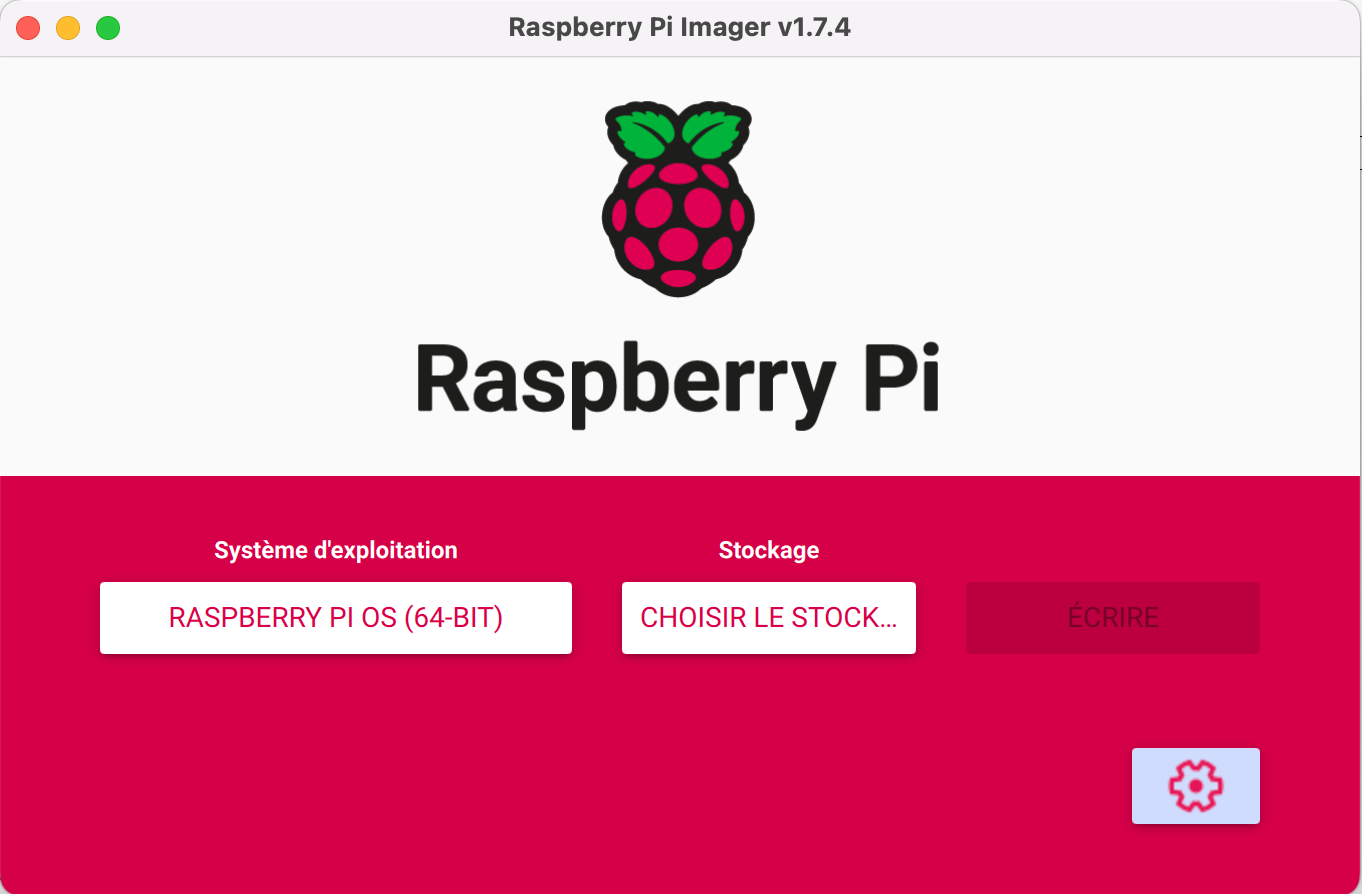
\includegraphics[width=\linewidth]{raspberrypi_imager}
						\caption{Menu}
						\label{fig:raspberrypiimager}
					\end{subfigure}
					\begin{subfigure}{0.49\textwidth}
						\centering
						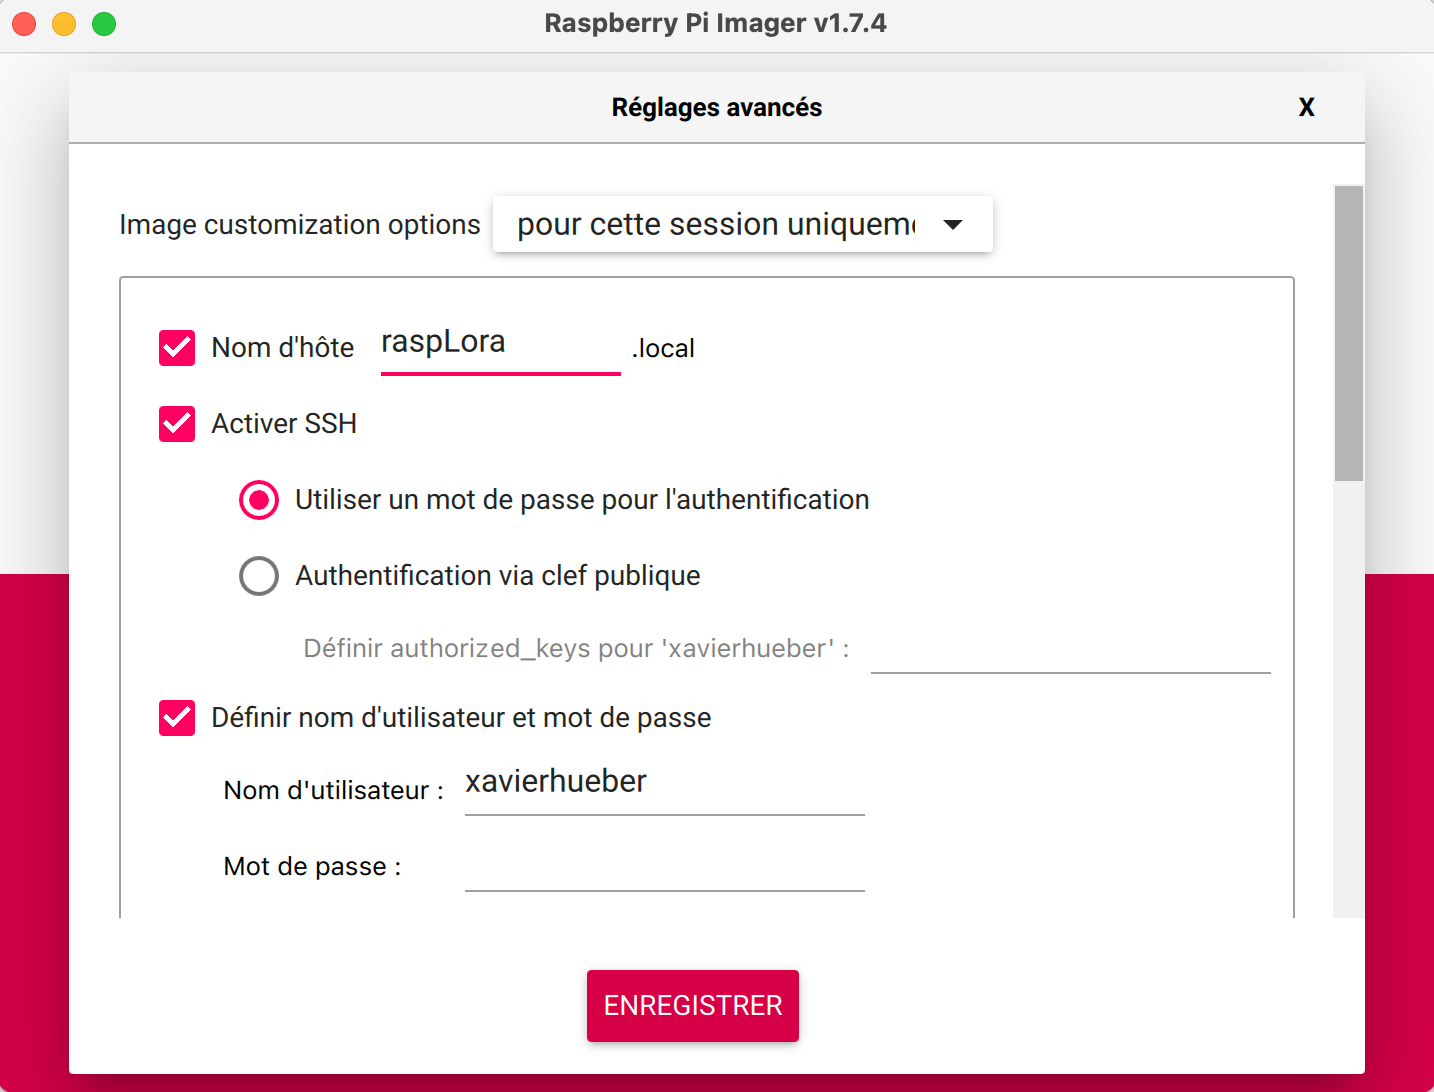
\includegraphics[width=\linewidth]{raspberrypi_imager1}
						\caption{Configuration du SSH et de l'utilisateur}
						\label{fig:raspberrypiimager1}
					\end{subfigure}
					\caption{Raspberry Pi Imager}
				\end{figure}
			\subsubsection{Logiciels tiers}
				Maintenant que nous avons installé un système d'exploitation sur le Raspberry Pi, nous pouvons installer une application pour récupérer et gérer les paquets LoRaWAN\textsuperscript\textregistered.
				
				Nous voulions pour cela installer l'application proposé par Seeed pour l'utilisation de leur HAT, cependant nous n'avons pas trouvé de liens de téléchargement ni de guide d'installation disponible sur leur site web. 
				Nous avons alors commencé par chercher des applications tierces compatible avec le module RHF0M301. Une solution simple était d'installer basicstation, un logiciel développé par TTN qui transfère tous les paquets vers leurs serveurs.
				
				Cependant, nous ne voulions pas pour commencer des tests, être dépendant de TTN et de leurs services (ceux-ci étant fortement limités à 30 secondes d'émission par jour).
				Nous avons alors décidé de chercher une autre solution et sommes tombés sur ChirpStack. ChirpStack est un ensemble d'applications permettant la réception, l'envoi et la gestion de paquets LoRaWAN\textsuperscript\textregistered. 
				
				
			\subsection{Installation de l'environnement de développement Espressif}
			
	\newpage
	\section{Sources}
		\printbibliography
\end{document}